\documentclass{beamer}
\usetheme{Madrid}
\usepackage{minted}
% sudo tlmgr install minted
\usepackage[utf8]{inputenc}
\usepackage[T2A]{fontenc}
\usepackage[russian,english]{babel}

% Footline: show current section (left) and frame numbers (right)
\setbeamertemplate{footline}{%
  \leavevmode%
  \hbox{%
    \begin{beamercolorbox}[wd=.78\paperwidth,ht=2.5ex,dp=1ex,left]{author in head/foot}%
      \hspace*{1em}\usebeamerfont{footline}\insertsectionhead%
    \end{beamercolorbox}%
    \begin{beamercolorbox}[wd=.22\paperwidth,ht=2.5ex,dp=1ex,right]{date in head/foot}%
      \usebeamerfont{footline}\insertframenumber{} / \inserttotalframenumber\hspace*{1em}%
    \end{beamercolorbox}%
  }%
}

\newcommand{\parpause}[1]{\only<+->{#1\par}}

\AtBeginSection[]
{
  \begin{frame}
    \frametitle{Содержание}
    \tableofcontents[currentsection]
  \end{frame}
}

\title{Семинар 3. Системная архитектура распределенных систем: Docker, Linux и т.п.}
\subtitle{Распределенные вычисления}
\author{Георгий Семенов}
\institute{Институт прикладных компьютерных наук \\ Университет ИТМО}
\date{весна 2026}

\begin{document}

\frame{\titlepage}

\begin{frame}
\frametitle{Организационные моменты}

\begin{itemize}
  \item Первое домашнее задание – жесткий дедлайн в 23:59 19.03.2026
  \begin{itemize}
    \item Всего 10 баллов: автотесты и корректность кода – допуск (ровно фиксированные 5 баллов), оцениваются ответы на вопросы от 0 до 5 баллов
    \item Ответы на вопросы должны быть подробными, с примерами и объяснениями, а не просто <<да>> или <<нет>>
    \item Учитывая невозможность проверить ответы на использование GPT, требования к качеству ответов высокие
    \item Если есть замечания, можно будет исправить в течение недели после дедлайна без потери баллов
    \item Для посылок после дедлайна – штраф $50 \%$
    \item (!) Не забывайте указать ФИО в своем Pull Request
  \end{itemize}
  \item Всего будет $\pm 5$ обязательных домашних заданий ($\pm 10$ баллов за каждое), которые будут выходить примерно раз в 2 недели
  \begin{itemize}
    \item \textbf{A -- <<5>>} – $\geq 90\%$ от общей суммы обязательных баллов
    \item \textbf{B/C -- <<4>>} – $\geq 75\%$ от общей суммы обязательных баллов
    \item \textbf{D/E -- <<3>>} – $\geq 60\%$ от общей суммы обязательных баллов
    \item \textbf{F -- <<2>>} – $< 60\%$ от общей суммы обязательных баллов
	\end{itemize}
\end{itemize}

\end{frame}

\section{Исполнение программы в ОС}

\begin{frame}
\frametitle{Как исполняется программа в ОС?}

\begin{itemize}
	\item Операционная система – управляет ресурсами вычислительного узла и предоставляет API {\itshape системных вызовов} для программ
	\begin{itemize}
        \item Поток – единица диспетчеризации для разделения CPU (int main())
        \item Виртуальная память – пространство динамически выделяемой памяти RAM (+swap) для программы (malloc/free)
        \item Сокет (ip + порт) – канал для обмена данными в рамках I/O
    \end{itemize}
    {\pause
    \item Что происходит, когда мы запускаем программу в Linux?
	\begin{itemize}
        \item Создание подпроцесса (fork) – рождение нового PID как копии родительского процесса
        \item Загрузка исполняемого файла в RAM для нового процесса (exec, секции ELF)
        \item При этом был резервирована память под stack, а динамическая память (heap) будет выделяться по мере необходимости с помощью системных вызовов
        \item Работа с памятью файлами, динамическими библиотеками, сокетами и т.п. – все через системные вызовы ОС (calling conventions)
    \end{itemize}
    }
\end{itemize}

\end{frame}

\begin{frame}
\frametitle{Какие неявные зависимости есть у программы?}

\begin{itemize}
	\item Порядок сборки – библиотеки, пакеты, интерфейсы и API ОС
	\item Исполняющая среда – непосредственно ОС, виртуальная машина, интерпретатор и т.п.
	\item Файлы, появляющиеся в процессе работы программы
	\begin{itemize}
        \item Stateful файлы – конфигурация, данные и т.п.
        \item Временные и мусорные файлы – AppData, /tmp, ~/.cache и т.п.
    \end{itemize}
    \item Сетевое окружение
    \begin{itemize}
        \item Открытые порты (сокеты) и их forwarding наружу
        \item Доступные IP-адреса сторонних сервисов и способ их адресации с помощью DNS
    \end{itemize}
\end{itemize}

\end{frame}

\section{Введение в Docker}

\begin{frame}
\frametitle{Что такое Docker и зачем он нужен?}

Docker – платформа для исполнения приложений в изолированных {\itshape контейнерах}.

\begin{itemize}
	\item Файл Dockerfile – декларативное описание процесса сборки образа (image) для контейнера
	\item В результате сборки образа по Dockerfile мы получаем {\itshape образ} (image), или несколько образов в случае multi-stage
    \item Мы можем запустить контейнер на основе образа, указывая дополнительные параметры:
    \begin{itemize}
        \item Отображение портов внутри контейнера на порты хоста (forwarding)
        \item Режимы сети (host, bridge, none) для обеспечения сетевой связности между контейнерам, хостом и внешним миром
        \item Volumes – можно примонтировать директории на хосте внутрь контейнера для обмена данными между ними (данные не удалятся, когда контейнер будет удален)
        \item Переменные окружения (environment) для передачи конфигурации внутрь контейнера
    \end{itemize}
\end{itemize}

\end{frame}

\begin{frame}[fragile]
\frametitle{Пример Dockerfile}

\begin{minted}[escapeinside=||]{dockerfile}
# ARG - Use build-time variables.
ARG RELEASE
# LABEL - Add metadata to an image.
LABEL org.opencontainers.image.ref.name=ubuntu
# ADD - Add local or remote files and directories.
ADD file ... in /
# CMD - Specify default commands.
CMD ["/bin/bash"] # Specify default commands.
# ENV - Set environment variables.
ENV JAVA_HOME=/opt/java/openjdk
# RUN - Execute build commands.
RUN /bin/sh -c set -eux;
# COPY - Copy files and directories.
COPY --chmod=755 entrypoint.sh /__cacert_entrypoint.sh
# ENTRYPOINT - Specify default executable.
ENTRYPOINT ["/__cacert_entrypoint.sh"]
\end{minted}

\end{frame}

\begin{frame}[fragile]
\frametitle{Пример Dockerfile (продолжение)}

\begin{minted}[escapeinside=||]{dockerfile}
# CMD - Specify default commands.
CMD ["jshell"]
# EXPOSE - Describe which ports your application is listening on.
EXPOSE [25565/tcp]
# VOLUME - Create volume mounts.
VOLUME [/data]
# WORKDIR - Change working directory,
WORKDIR /data
# STOPSIGNAL - Specify the system call signal for exiting a container.
STOPSIGNAL SIGTERM
# HEALTHCHECK - Check a container's health on startup.
HEALTHCHECK &{["CMD-SHELL" "mc-health"] "30s" "0s"
\end{minted}

\end{frame}

\begin{frame}[fragile]
\frametitle{Как собрать образ и запустить контейнер?}

\begin{minted}[escapeinside=||]{bash}
# . - директория, где лежит Dockerfile, т.е. текущая
docker build -t minecraft-server .

# посмотреть локальные образы
docker image ls

# -d - запуск в фоновом режиме (detached)
# -p - port forwarding: отображаем порт 25565 на хост
docker run -d -p 127.0.0.1:25565:25565 minecraft-server

# посмотреть контейнеры
docker ps
\end{minted}

\end{frame}

\begin{frame}[fragile]
\frametitle{Пример docker-compose.yaml}

\begin{minted}[escapeinside=||]{yaml}
services:
  minecraft: # название контейнера (сервиса)
    image: itzg/minecraft-server:latest # имя образа и тэг
    pull_policy: daily # как часто обновлять образ
    tty: true
    stdin_open: true
    ports: # отображаем внутр. порт 25565 на порт хоста 25565
      - "25565:25565"
    environment: # конфигурируем через переменные окружения
      EULA: "TRUE"
      VERSION: "1.21.11"
      SERVER_NAME: "Уютные зимние приключения"
      DIFFICULTY: normal
    volumes: # монтируем директорию на хосте внутрь
             # контейнера для сохранения данных
      - ./data:/data
\end{minted}

\end{frame}

\begin{frame}[fragile]
\frametitle{Как собрать образ и запустить контейнер?}

\begin{minted}[escapeinside=||]{bash}
# в директории, где лежит docker-compose.yaml
docker compose up -d

docker compose stop # (1) просто остановим все
docker compose down # ИЛИ (2): еще и грохнем контейнеры и т.п.
\end{minted}

\end{frame}


\begin{frame}
\frametitle{Discussion: что для нас Docker?}

\begin{itemize}
	\item Docker - среда виртуализации для исполнения программ в изолированных контейнерах
	\item Внутри каждого контейнера запущена своя ОС (обычно Linux)
	\begin{itemize}
    \item Ядро ОС резидентно, т.е. должно лежать в оперативной памяти хоста, поэтому важен размер
    \item Alpine Linux – 5 MB по образу
  \end{itemize}
	\item Docker свойственно захватывать ресурсы хоста
  \begin{itemize}
    \item RAM - эмулирует виртуальную память для контейнера, выделяя её из общей памяти хоста
    \item Firewall - Docker управляет iptables в Linux (использовать совместно с ufw - не стоит)
  \end{itemize}
  \item Какие плюсы и минусы Docker?
  \begin{itemize}
    \item (+) Декларативная абстракция для описания сред для сборки и запуска программ
    \item (-) Ненулевые издержки на RAM
  \end{itemize}
\end{itemize}

\end{frame}

\begin{frame}
\frametitle{Docker vs Виртуальная машина}

\begin{itemize}
  \item Виртуальная машина (VM):
  \begin{itemize}
    \item Полная эмуляция оборудования – запущена отдельная ОС с собственным ядром
    \item Медленный старт – стартует как отдельный компьютер
    \item Полная изоляция – VM не видят друг друга на уровне ОС
  \end{itemize}
  \item Docker контейнер:
  \begin{itemize}
    \item Легковесная виртуализация – все контейнеры используют одно ядро хоста (namespaces + cgroups)
    \item Малый overhead – контейнеры занимают мегабайты, не gigabytes
    \item Изоляция на уровне процессов – видн друг друга в сети, но не при доступе к файловой системе
  \end{itemize}
  \item Вывод: Docker идеален для микросервисов, VM – для полной изоляции и различных ОС
\end{itemize}

\end{frame}

\section{Ликбез по Linux}

\begin{frame}
\frametitle{Какие свойства мы имеем в виду, говоря о Linux?}

\begin{itemize}
	\item Свободный, модульный и открытый код ОС и программ (copy-left лицензия GPL)
	\item Де факто промышленный стандарт: POSIX-совместимость, стандартные C-headers, ELF, .so и т.п.
	\item Декларативные способы решения задач по системному администрированию (в т.ч. DevOps)
\end{itemize}

\end{frame}

\begin{frame}
\frametitle{Что нужно обязательно представлять о Linux?}

\begin{itemize}
	\item Файловая система в Linux-системах
  \begin{itemize}
    \item Все – это файл (включая устройства, сокеты и т.п.)
    \item Иерархическая структура файловой системы (root, /home, /dev, /proc и т.п.)
    \item Узлы иерархической структуры - inodes, ссылаются на блоки данных
    \item Права доступа к файлам: владелец (u), группа (g), остальные (o); чтение (r), запись (w), выполнение (x)
  \end{itemize}
  \item Порядок инициализации и управления ОС
  \begin{itemize}
    \item Базово о физическом запуске - BIOS/UEFI, загрузчик (GRUB), ядро ОС, init-система (systemd)
    \item Service в Linux: юнит, который может быть запущен, остановлен, перезапущен и т.п. с помощью systemctl
    \item Процессы и демоны – top, htop, ps, systemctl status и т.п.
    \item Пользователи и группы - useradd, groupadd, passwd и т.п.
  \end{itemize}
\end{itemize}

\end{frame}

\begin{frame}
\frametitle{Управление доступом к файлам}

\begin{center}
  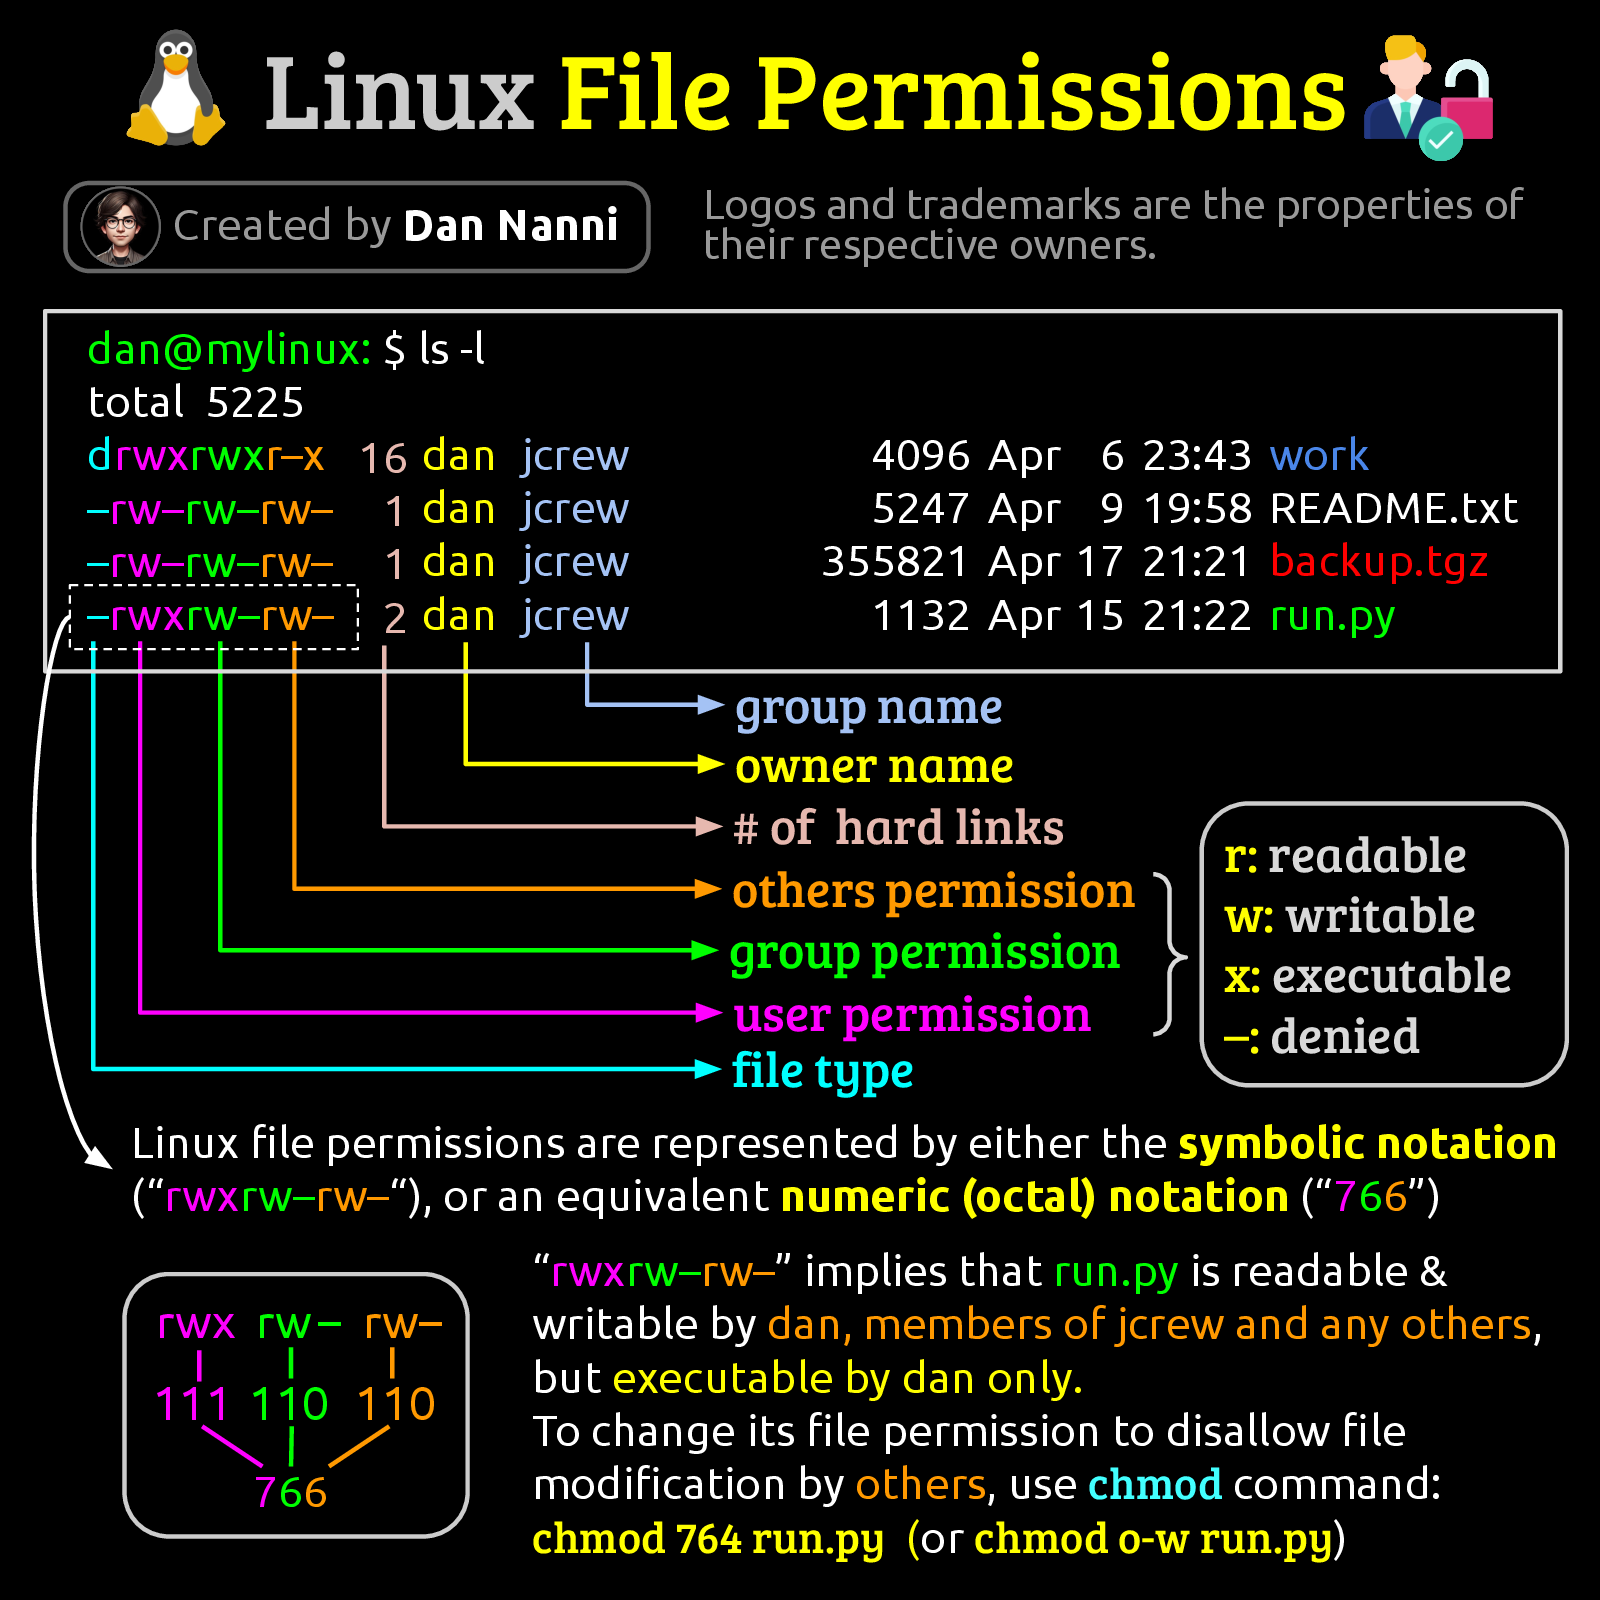
\includegraphics[width=0.8\linewidth,keepaspectratio]{images/linuxfilepermissions.png}
\end{center}

\end{frame}

\begin{frame}
\frametitle{Загрузка сервисов}

\begin{center}
  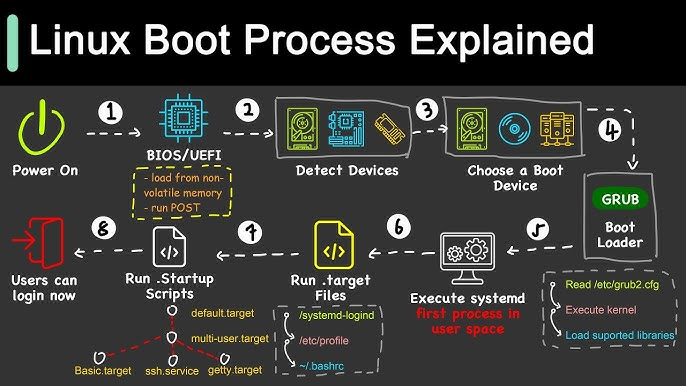
\includegraphics[width=1.0\linewidth,keepaspectratio]{images/linuxbootprocess.jpg}
\end{center}

\end{frame}

\begin{frame}
\frametitle{SSH-клиент}

\begin{itemize}
  \item SSH (Secure Shell) – протокол для безопасного удалённого доступа к машинам
  \begin{itemize}
    \item Аутентификация: пароль или публичный ключ (более безопасно)
    \item Шифрование трафика: все данные передаются в зашифрованном виде
    \item Туннелирование: можно проксировать трафик через SSH (port forwarding)
  \end{itemize}
  \item Подключение к серверу:
  \begin{itemize}
    \item \texttt{ssh user@host} – базовое подключение
    \item \texttt{ssh -i /path/to/key user@host} – с использованием приватного ключа
    \item \texttt{ssh -p 2222 user@host} – подключение на нестандартный порт
  \end{itemize}
  \item Генерация пары ключей:
  \begin{itemize}
    \item \texttt{ssh-keygen -t ed25519 -f ~/.ssh/id\_ed25519}
    \item Копирование публичного ключа на сервер: \texttt{ssh-copy-id -i ~/.ssh/id\_ed25519.pub user@host}
  \end{itemize}
\end{itemize}

\end{frame}

\begin{frame}
\frametitle{SSH-сервер}

\begin{itemize}
  \item Конфигурация в \texttt{/etc/ssh/sshd\_config}:
  \begin{itemize}
    \item \texttt{Port 22} – порт для слушания (лучше менять на нестандартный)
    \item \texttt{PermitRootLogin no} – запретить вход под root (обязательно!)
    \item \texttt{PasswordAuthentication no} – разрешить только аутентификацию по ключам
    \item \texttt{PubkeyAuthentication yes} – включить аутентификацию по публичным ключам
    \item \texttt{PermitEmptyPasswords no} – запретить пустые пароли
    \item \texttt{X11Forwarding no} – отключить X11 forwarding для безопасности
  \end{itemize}
  \item Запуск и управление:
  \begin{itemize}
    \item \texttt{systemctl restart sshd} – перезапустить сервис после изменения конфига
    \item \texttt{systemctl status sshd} – проверить статус
    \item \texttt{ss -tlnp | grep ssh} – проверить, что сервер слушает на нужном порту
  \end{itemize}
  \item Хранение публичных ключей клиентов: \texttt{~/.ssh/authorized\_keys}
\end{itemize}

\end{frame}

\begin{frame}
\frametitle{Упражнения (опциональные)}

\begin{enumerate}
  \item Создать папку (mkdir, -p) с файлами (touch, nano) и гранулярно настроить права доступа к ним (chmod, chown)
     под произвольную бизнес-задачу (например, для файлов веб-сервера - менять можем мы, но не он)
  \item Создать service (service-файл) в Linux, который будет запускаться в качестве демона проверки состояния системы (скрипт на Bash) 
  и логировать раз в какое-то время результаты в файл (systemctl list-dependencies, status, logs и т.п.)
  \item Установить Docker, запустить произвольный сервис с помощью docker-compose:
  \begin{itemize}
    \item nginx-сервер (проверить можно, открыв в браузере http://localhost:80)
    \item Postgres (проверить, подключившись через psql, DataGrip и т.п.)
    \item Minecraft-сервер (проверить можно, если есть игра)
  \end{itemize}
\end{enumerate}

\end{frame}

\section{Микросервисная архитектура}

\begin{frame}{Что такое монолитная архитектура?}

Монолитная архитектура – архитектурный стиль, при котором все компоненты приложения тесно связаны и развертываются как единое целое:

\begin{itemize}
\item (+) Простота разработки и развертывания – все в одном месте
\item (-) Сложность масштабирования – масштабируем все целиком, даже если нужно масштабировать только часть
\item (-) Сложность поддержки – изменения в одной части могут повлиять на другие части, что усложняет отладку и тестирование
\item (-) Огромный монорепозиторий – трудно вмержить изменения, если команда большая
\item (-) Фиксация на одном языке программирования и стеке
\end{itemize}

Например, 'Монолит' в VK – исполняемый файл (kPHP) размером в $\approx 1.5 GB$

\end{frame}

\begin{frame}{Постерный доклад на примере Google Cloud}

\begin{center}
  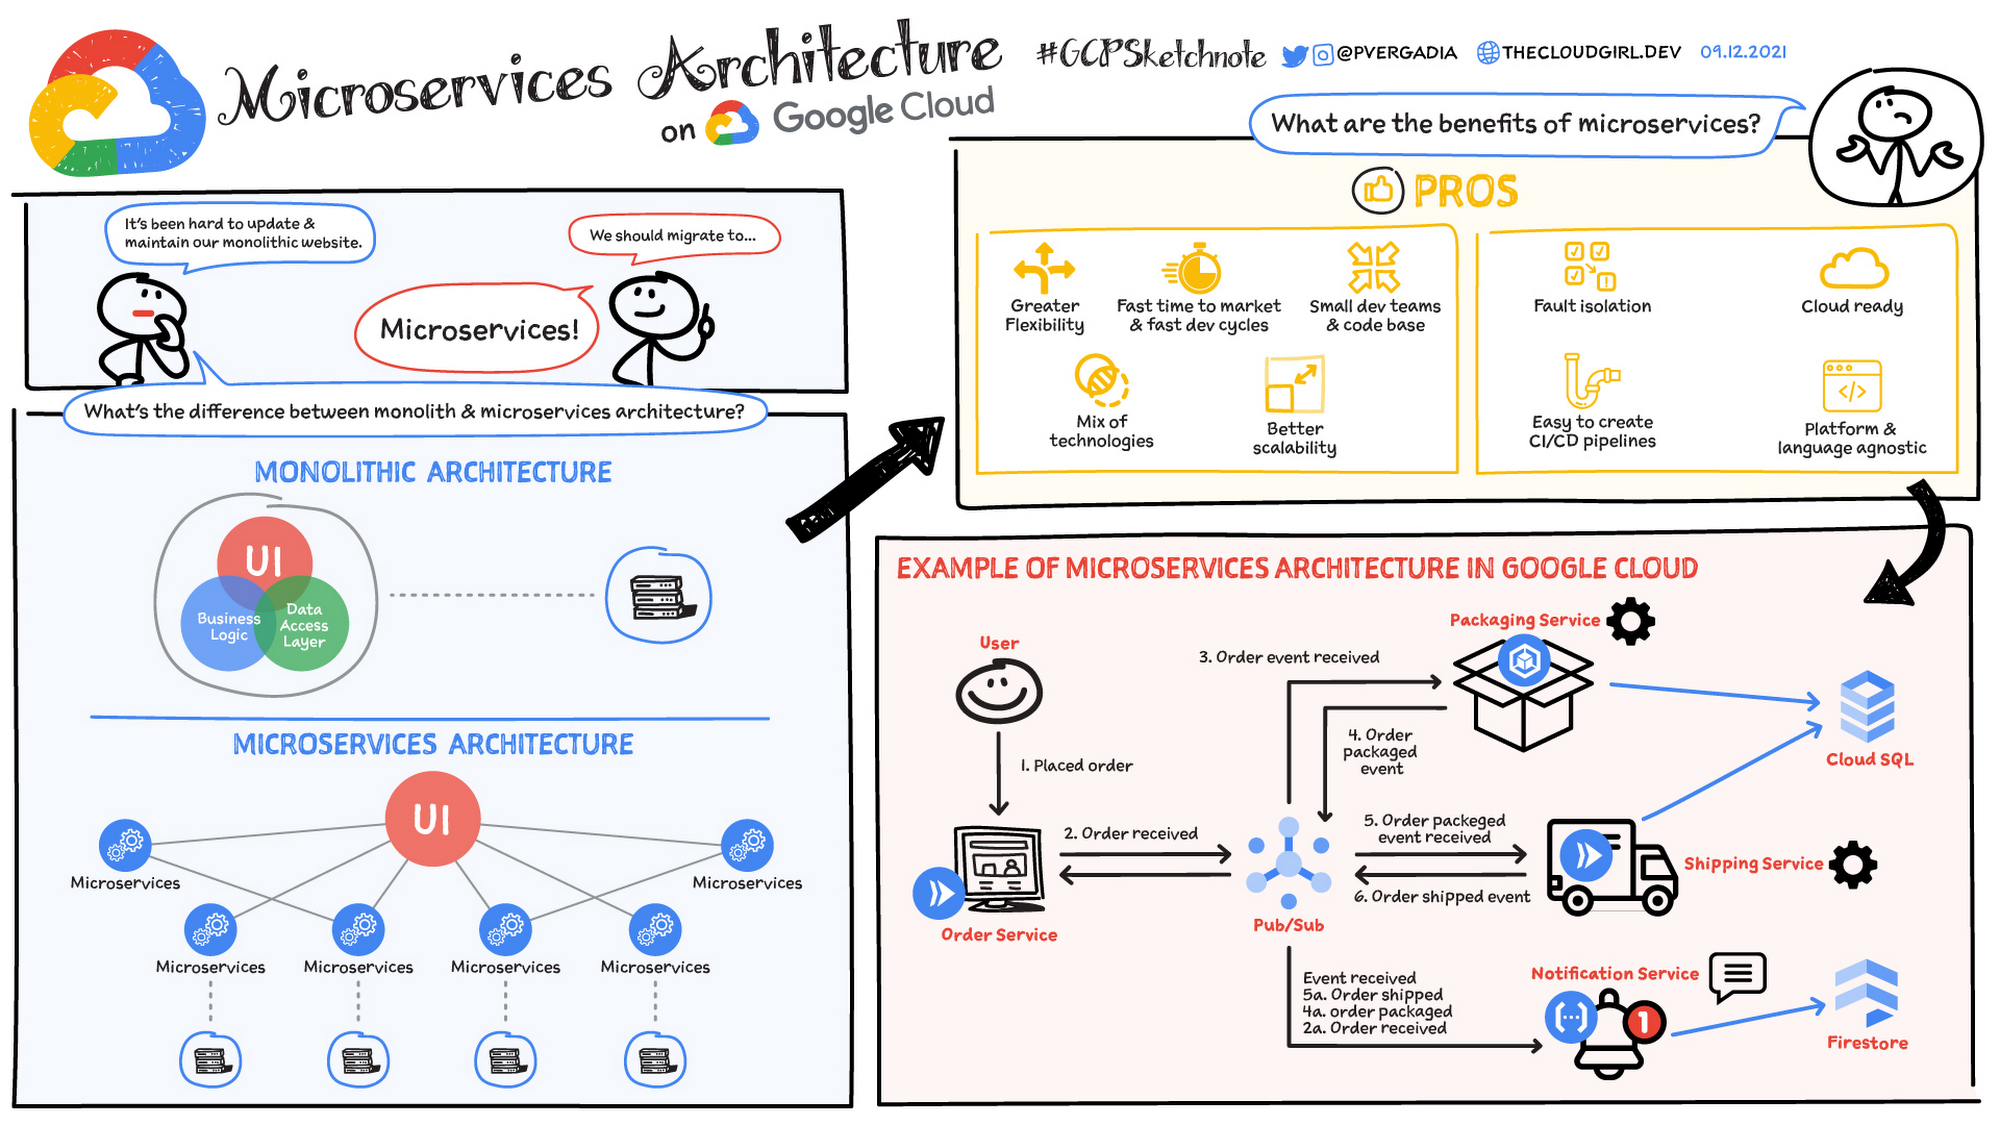
\includegraphics[width=1.0\linewidth,keepaspectratio]{images/google_cloud_microservices.png}
\end{center}

\end{frame}

\begin{frame}{Что такое микросервисная архитектура?}

Микросервисная архитектура – архитектурный стиль, при котором приложение декомпозируется на микросервисы:

\begin{itemize}
\item Микросервис – автономный сервис, соответствующий одной бизнес-функции (со своим хранилищем)
\item Разрабатывается независимо от других микросервисов, хорошо масштабируется
\item Соединяется с другими микросервисами через HTTP/REST, gRPC, шины сообщений (Kafka, RabbitMQ) и т.п.
\end{itemize}

\end{frame}

\begin{frame}{Микросервисы как узлы распределенной системы}

\begin{itemize}
\item Экземпляры микросервиса – {\bfseries поды} – горизонтально масштабируются в зависимости от внешней нагрузки
\item Состав подов динамический – может меняться в процессе работы, что требует динамической маршрутизации и балансировки нагрузки
\item Обязательно найдутся поды, которые будут работать некорректно (crash, memory leak, network issues и т.п.), поэтому
      требуется отказоустойчивость, а распределенные алгоритмы должны это учитывать
\end{itemize}

\end{frame}

\section{Немного о Kubernetes}

\begin{frame}
\frametitle{Что такое Kubernetes?}

Kubernetes (K8s) – система оркестрации контейнеров с открытым исходным кодом для автоматизации развертывания, масштабирования и управления контейнеризованными приложениями.

\begin{itemize}
  \item Автоматическое развертывание подов на основе нагрузки и ограничений ресурсов
  \item Самовосстановление – перезапуск упавших контейнеров, замена недоступных подов
  \item Балансировка нагрузки и сетевая маршрутизация между подами (Service, Ingress)
  \item Хранение и управление секретами (пароли, токены, конфиги)
  \item Откат к предыдущим версиям (Deployment, ReplicaSet)
\end{itemize}

\end{frame}

\begin{frame}{Kubernetes как IaC инструмент}

\begin{center}
  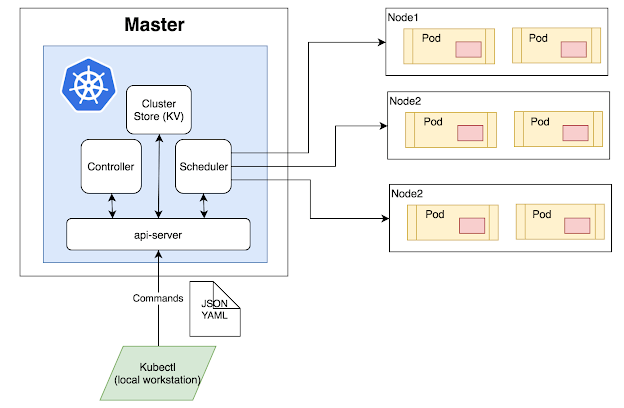
\includegraphics[width=1.0\linewidth,keepaspectratio]{images/kubernetes.png}
\end{center}

\end{frame}

\begin{frame}
\frametitle{Архитектура Kubernetes}

\begin{itemize}
  \item Control Plane – управляет состоянием кластера:
  \begin{itemize}
    \item API Server – REST API для управления ресурсами
    \item etcd – распределённое хранилище конфигурации и состояния
    \item Scheduler – распределяет поды на ноды
    \item Controller Manager – контроллеры для управления Deployment, Service и т.п.
  \end{itemize}
  \item Worker Nodes – исполняют поды:
  \begin{itemize}
    \item kubelet – агент на ноде, взаимодействует с Control Plane
    \item Container Runtime – Docker, containerd, CRI-O и т.п.
  \end{itemize}
\end{itemize}

\end{frame}

\begin{frame}[fragile]
\frametitle{Пример манифеста Kubernetes (Deployment)}

\begin{minted}[escapeinside=||]{yaml}
apiVersion: apps/v1
kind: Deployment
metadata:
  name: nginx-deployment
spec:
  replicas: 3 # запустить 3 экземпляра
  selector:
  matchLabels:
    app: nginx
  template:
  metadata:
    labels:
    app: nginx
  spec:
    containers:
    - name: nginx
    image: nginx:1.14.2
    ports:
    - containerPort: 80
    resources:
      limits:
      memory: "128Mi"
      cpu: "500m"
\end{minted}

\end{frame}

\begin{frame}[fragile]
\frametitle{Основные команды kubectl}

\begin{minted}[escapeinside=||]{bash}
# Применить манифест
kubectl apply -f deployment.yaml

# Получить состояние подов
kubectl get pods -n default

# Просмотреть логи пода
kubectl logs <pod-name> -f

# Выполнить команду внутри пода
kubectl exec -it <pod-name> -- /bin/bash

# Просмотреть описание ресурса
kubectl describe deployment nginx-deployment

# Удалить ресурс
kubectl delete deployment nginx-deployment
\end{minted}

\end{frame}

\section{Немного об Ansible}

\begin{frame}
\frametitle{Что такое Ansible?}

Ansible – инструмент для автоматизации управления конфигурацией и развертывания приложений на удалённых машинах.

\begin{itemize}
  \item Agentless: не требует установки агента на целевых машинах, использует SSH
  \item Декларативный подход: описываем желаемое состояние, Ansible приводит систему в это состояние
  \item Идемпотентность: повторное выполнение playbook не вызывает нежелательных побочных эффектов
  \item Инвентарь (inventory) – список хостов и групп для управления
  \item Playbook – YAML-файл с последовательностью задач (tasks)
  \item Vault – для хранения секретов
\end{itemize}

\end{frame}

\begin{frame}{Ansible как IaC инструмент}

\begin{center}
  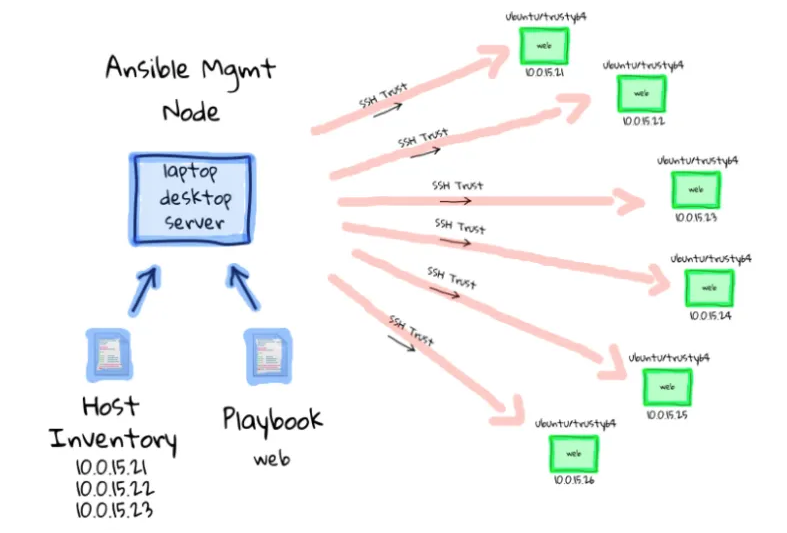
\includegraphics[width=1.0\linewidth,keepaspectratio]{images/ansible.png}
\end{center}

\end{frame}

\begin{frame}[fragile]
\frametitle{Структура Ansible проекта}

\begin{minted}{text}
ansible-project/
|-- inventory.yaml          # список хостов
|-- playbook.yaml          # основной playbook
|-- roles/
|   |-- webserver/
|   |   |-- tasks/
|   |   |   `-- main.yaml  # задачи роли
|   |   |-- templates/     # шаблоны файлов
|   |   `-- vars/
|   |       `-- main.yaml  # переменные роли
|   `-- database/
|       `-- ...
`-- group_vars/
    `-- webservers.yaml    # переменные группы
\end{minted}

\end{frame}

\begin{frame}[fragile]
\frametitle{Пример inventory.yaml}

\begin{minted}[escapeinside=||]{yaml}
all:
  children:
  webservers:
    hosts:
    web1:
      ansible_host: 192.168.1.10
      ansible_user: ubuntu
    web2:
      ansible_host: 192.168.1.11
      ansible_user: ubuntu
  databases:
    hosts:
    db1:
      ansible_host: 192.168.1.20
      ansible_user: ubuntu
\end{minted}

\end{frame}


\begin{frame}[fragile]
\frametitle{Понятия в playbook.yaml}

\begin{itemize}
  \item \textbf{Task} – атомарная единица работы, которая выполняет одно действие (установка пакета, копирование файла, запуск команды и т.п.)
  \begin{itemize}
    \item Задачи группируются в playbook или роль
    \item Каждая task может иметь условия (when), циклы (loop) и зависимости (dependencies)
  \end{itemize}
  
  \item \textbf{Role} – переиспользуемый набор файлов (tasks, handlers, templates, vars, files и т.п.) для выполнения конкретной функции
  \begin{itemize}
    \item Инкапсулирует логику управления конфигурацией (например, роль \texttt{webserver} содержит все необходимое для установки и настройки веб-сервера)
    \item Позволяет избежать дублирования кода и облегчает переиспользование в разных playbook'ах
  \end{itemize}
  
  \item \textbf{Handler} – специальный вид task, который выполняется только при срабатывании события \texttt{notify}
  \begin{itemize}
    \item Обычно используется для перезапуска сервисов при изменении конфигурационных файлов
    \item Гарантирует, что сервис перезапустится только один раз, даже если несколько task'ов вызовут один и тот же handler
  \end{itemize}
\end{itemize}

\end{frame}

\begin{frame}[fragile]
\frametitle{Пример playbook.yaml}


\begin{columns}[T]
\column{0.5\textwidth}
\begin{minted}[escapeinside=||,fontsize=\small]{yaml}
---
- name: Deploy web application
  hosts: webservers
  become: yes
  roles:
  - webserver
  tasks:
  - name: Install nginx
    apt:
    name: nginx
    state: present
\end{minted}

\column{0.5\textwidth}
\begin{minted}[escapeinside=||,fontsize=\small]{yaml}
  - name: Copy nginx config
    template:
    src: nginx.conf.j2
    dest: /etc/nginx/nginx.conf
    notify: restart nginx
    
  handlers:
  - name: restart nginx
    service:
    name: nginx
    state: restarted
\end{minted}
\end{columns}

\end{frame}

\begin{frame}[fragile]
\frametitle{Основные команды Ansible}

\begin{minted}[escapeinside=||]{bash}
# Выполнить ad-hoc команду на всех хостах
ansible all -i inventory.yaml -m ping

# Выполнить playbook
ansible-playbook -i inventory.yaml playbook.yaml

# Выполнить playbook в режиме сухого прогона (check)
ansible-playbook -i inventory.yaml playbook.yaml --check

# Выполнить с повышенными привилегиями (become)
ansible-playbook -i inventory.yaml playbook.yaml -K

# Фильтровать по тегам
ansible-playbook -i inventory.yaml playbook.yaml -t deploy
\end{minted}

\end{frame}

\section{Немного о Terraform}

\begin{frame}
\frametitle{Что такое Terraform?}

Terraform – инструмент Infrastructure as Code (IaC) для описания и управления облачной инфраструктурой декларативным способом.

\begin{itemize}
  \item Provider – плагин для взаимодействия с облачным провайдером (AWS, GCP, Azure, Yandex Cloud и т.п.)
  \item Resource – примитивная единица инфраструктуры (VM, сеть, диск, RDS и т.п.)
  \item State – текущее состояние инфраструктуры (хранится локально или в удалённом backend)
  \item Plan – предварительный просмотр изменений перед применением
  \item Apply – применение плана для создания/изменения/удаления ресурсов
\end{itemize}

\end{frame}

\begin{frame}{Terraform как IaC инструмент}

\begin{center}
  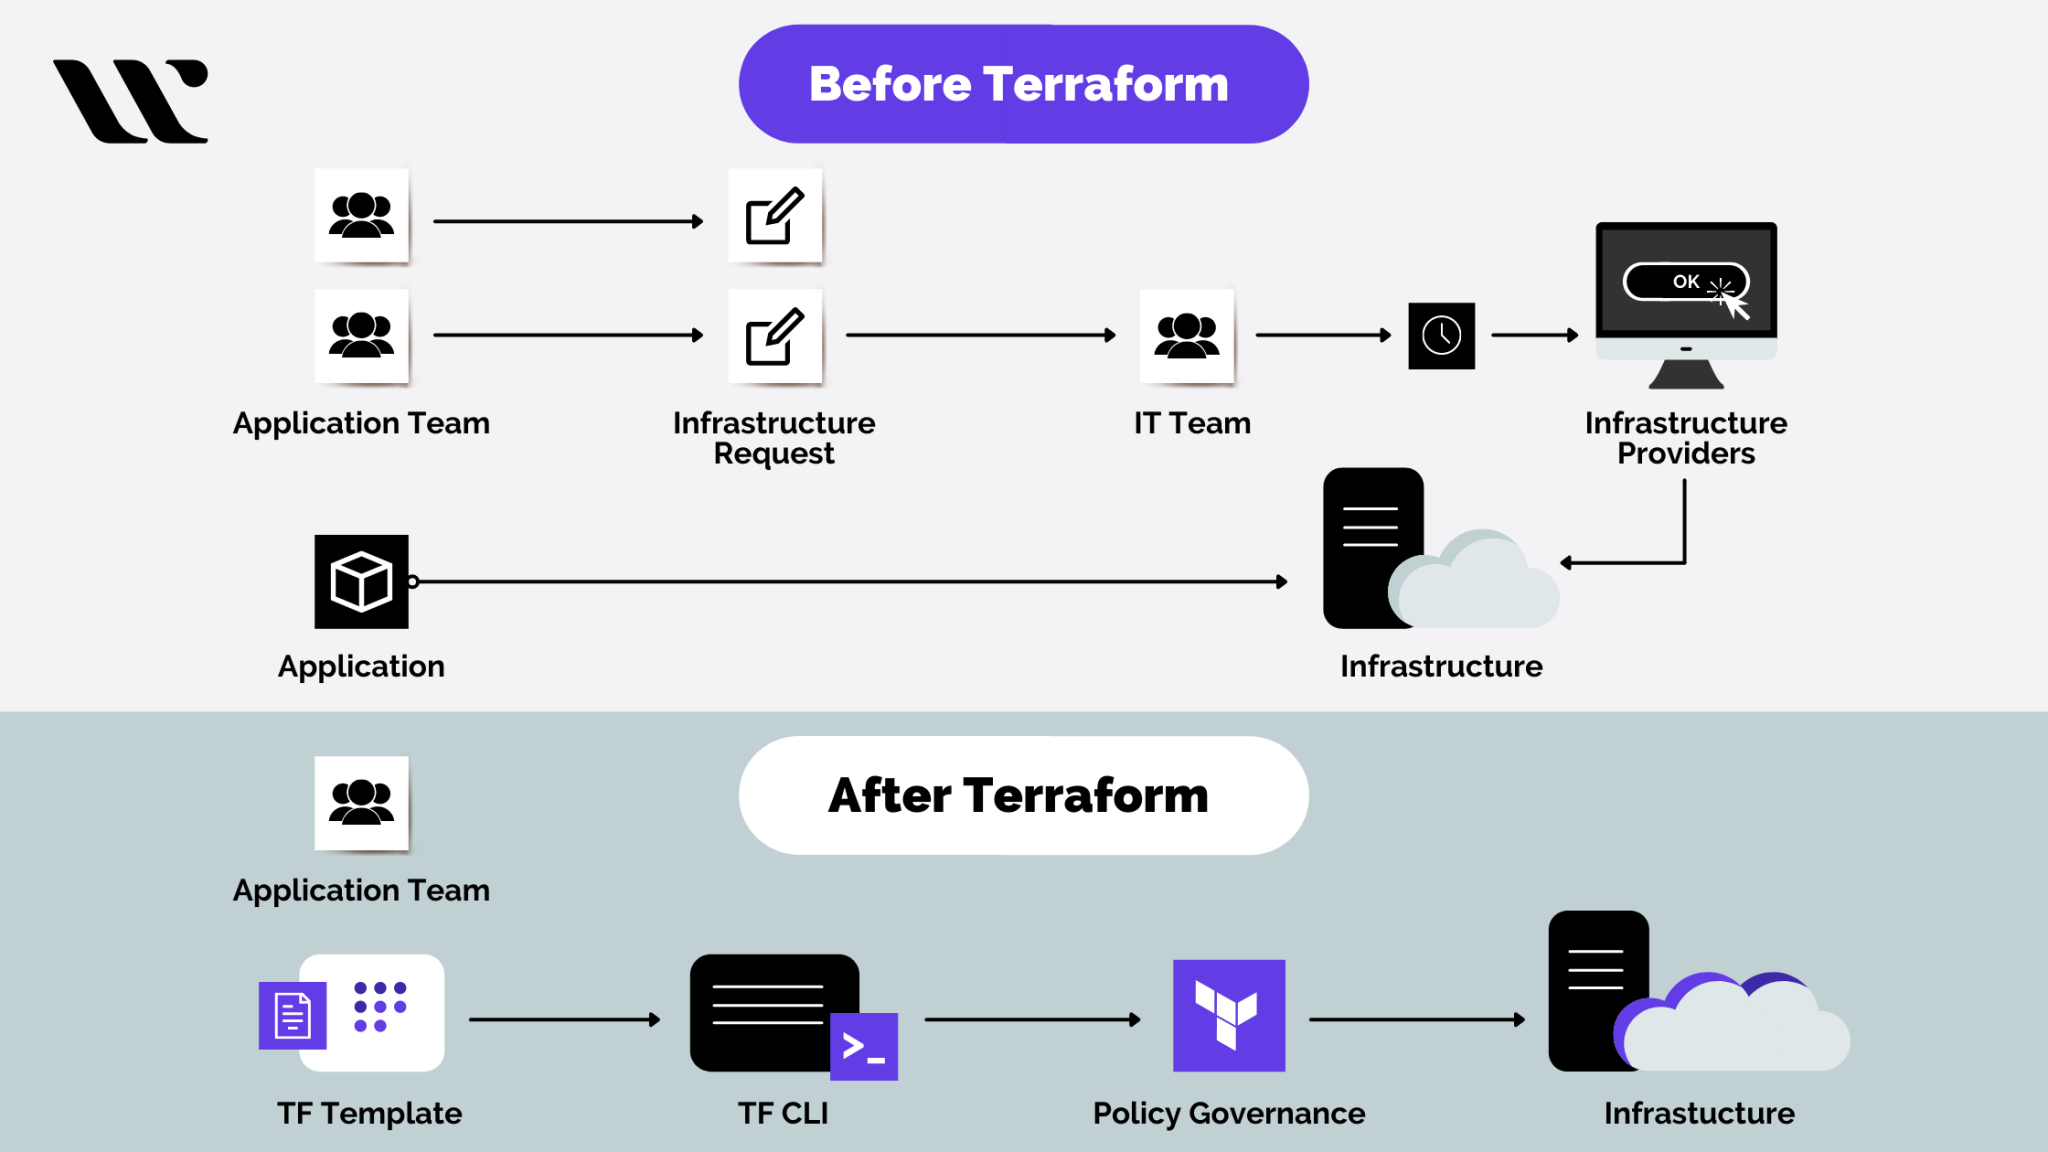
\includegraphics[width=1.0\linewidth,keepaspectratio]{images/terraform-intro.png}
\end{center}

\end{frame}

\begin{frame}
\frametitle{Основные концепции Terraform}

\begin{itemize}
  \item \textbf{Provider} – плагин для взаимодействия с облачным провайдером или сервисом (AWS, GCP, Azure, Yandex Cloud, Kubernetes и т.п.)
  \begin{itemize}
    \item Определяется в блоке \texttt{provider} с указанием региона, учётных данных и другых параметров
  \end{itemize}
  
  \item \textbf{Resource} – объект инфраструктуры, управляемый провайдером (виртуальная машина, сеть, хранилище, база данных и т.п.)
  \begin{itemize}
    \item Каждый ресурс имеет тип (например, \texttt{aws\_instance}) и имя для идентификации
  \end{itemize}
  
  \item \textbf{Variable} – входной параметр конфигурации Terraform для параметризации и переиспользования кода
  \begin{itemize}
    \item Может иметь тип (\texttt{string}, \texttt{number}, \texttt{list}, \texttt{map}), значение по умолчанию и описание
  \end{itemize}
  
  \item \textbf{Output} – выходное значение, которое выводится после применения конфигурации (IP адреса, идентификаторы ресурсов и т.п.)
  \begin{itemize}
    \item Используется для передачи значений между модулями или для вывода информации пользователю
  \end{itemize}
  
  \item \textbf{Ingress} – ресурс Kubernetes для управления входящим трафиком к сервисам внутри кластера
  \begin{itemize}
    \item Определяет правила маршрутизации HTTP/HTTPS трафика на основе хоста и пути
  \end{itemize}
\end{itemize}

\end{frame}

\begin{frame}{Terraform как IaC инструмент}

\begin{center}
  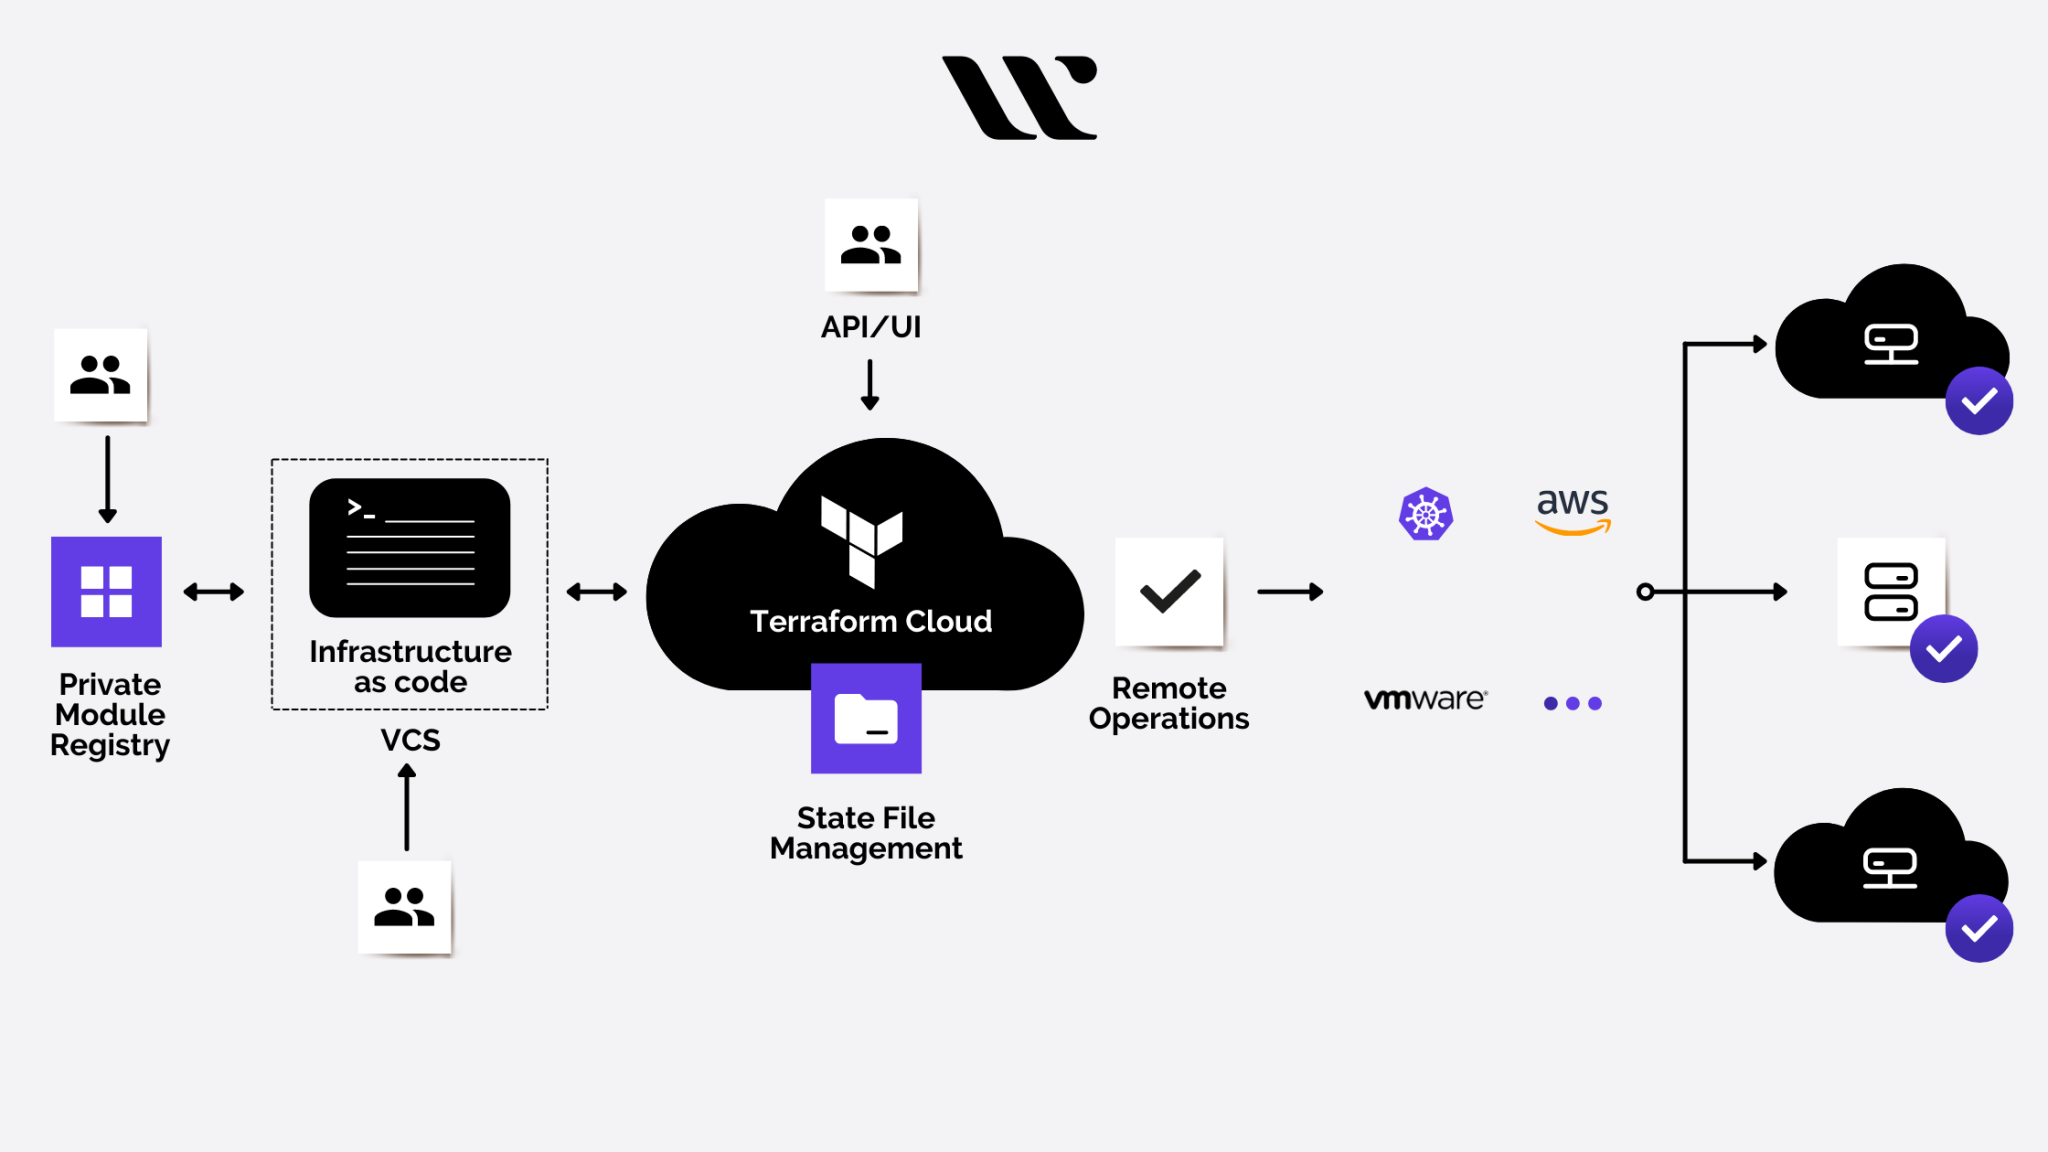
\includegraphics[width=1.0\linewidth,keepaspectratio]{images/terraform-edits.png}
\end{center}

\end{frame}

\begin{frame}[fragile]
\frametitle{Пример конфигурации Terraform}

\begin{columns}[T]
\column{0.45\textwidth}
\begin{minted}[escapeinside=||,fontsize=\small]{hcl}
terraform {
  required_providers {
    aws = {
      source  = "hashicorp/aws"
      version = "~> 5.0"
    }
  }
}

provider "aws" {
  region = "us-east-1"
}
\end{minted}

\column{0.45\textwidth}
\begin{minted}[escapeinside=||,fontsize=\small]{hcl}
resource "aws_instance" "web" {
  ami           = "ami-0c55b159cbfafe1f0"
  instance_type = "t2.micro"
  vpc_security_group_ids = 
    [aws_security_group.web.id]
  tags = { Name = "web-server" }
}

resource "aws_security_group" "web" {
  name = "web-sg"
  ingress {
    from_port   = 80
    to_port     = 80
    protocol    = "tcp"
    cidr_blocks = ["0.0.0.0/0"]
  }
}
\end{minted}
\end{columns}

\end{frame}



\begin{frame}[fragile]
\frametitle{Переменные и выходные значения в Terraform}

\begin{minted}[escapeinside=||]{hcl}
variable "instance_count" {
  type        = number
  default     = 2
  description = "Количество инстансов"
}

variable "instance_type" {
  type    = string
  default = "t2.micro"
}

output "instance_ips" {
  value       = aws_instance.web[*].private_ip
  description = "Приватные IP адреса инстансов"
}
\end{minted}

\end{frame}

\begin{frame}[fragile]
\frametitle{Основные команды Terraform}

\begin{minted}[escapeinside=||]{bash}
# Инициализация рабочей директории
terraform init

# Форматирование конфигурации
terraform fmt

# Валидация синтаксиса
terraform validate

# Просмотр плана изменений
terraform plan

# Применение плана
terraform apply

# Вывести текущее состояние
terraform show

# Удалить ресурсы
terraform destroy
\end{minted}

\end{frame}

\begin{frame}
\frametitle{Module — переиспользуемые компоненты}

\begin{itemize}
  \item Module – инкапсулированный набор ресурсов Terraform для повторного использования
  \item Локальные модули – в пределах проекта (./modules/vpc, ./modules/rds)
  \item Удалённые модули – из Terraform Registry или git-репозитория
  \item Параметризация – передача входных переменных в модуль, получение выходных значений
\end{itemize}

Пример использования модуля:
\begin{itemize}
  \item \texttt{module "vpc" { source = "./modules/vpc", cidr\_block = "10.0.0.0/16" }}
  \item Обращение к выходу: \texttt{module.vpc.vpc\_id}
\end{itemize}

\end{frame}

\begin{frame}
\frametitle{Упражнения (опциональные)}

\begin{enumerate}
  \item Поднять локальный minikube-кластер, запустить Docker-контейнеры с ssh-агентами, настроить их через Ansible (hosts, playbooks)
  \item Реализовать \href{https://developer.hashicorp.com/terraform/tutorials/kubernetes/kubernetes-provider}{terraform-конфигурацию} для настройки локального kubernetes-кластера для нескольких подов с nginx-балансировщиками
  \item Поднять Kafka и сконфигурировать ее очереди и пользователей с помощью Terraform
  \item Реализовать Kubernetes Deployment/Job с sidecar-контейнером для логирования/prometheus/nginx для основного контейнера
  \item Снимаем для себя VPS-сервер с помощью хостинга и пишем для него ansible-конфигурацию для развертывания всего, что нам хочется (обращаем внимание на секреты и безопасность)
\end{enumerate}

\end{frame}

\begin{frame}{Итоги}

\begin{itemize}
\item Обсудили инфраструктурные аспекты исполнения узлов в распределенных системах
\item Выдано первое домашнее задание о часах и алгоритмах синхронизации
\end{itemize}

\end{frame}


\end{document}